%% =============================================================================
%%  Justificacion de la optimizacion: como se hizo y por que se eligio FLC-O.
%%  Documento de apoyo para la revision del articulo (no es el articulo). Compilar con pdfLaTeX + BibTeX.
%%  Las cifras salen de numeros.tex (gen_tablas_opt.py) y de justificacion_datos.tex / tabla_j_modelos.tex
%%  (gen_justificacion.py), ambos generados desde resultados/opt/*.json: nada se escribe a mano.
%% =============================================================================
\documentclass[11pt,a4paper]{article}
\usepackage[utf8]{inputenc}
\usepackage[T1]{fontenc}
\usepackage[spanish,es-tabla,es-nodecimaldot]{babel}
\addto\captionsspanish{\renewcommand{\figurename}{Fig.}}
\usepackage[a4paper,margin=2.1cm]{geometry}
\usepackage{amsmath,amssymb}
\usepackage{graphicx}
\usepackage{booktabs}
\usepackage{array}
\usepackage[table]{xcolor}
\usepackage{enumitem}
\usepackage{url}
\usepackage[colorlinks=true,linkcolor=blue!50!black,citecolor=blue!50!black,urlcolor=blue!50!black]{hyperref}
\graphicspath{{figures/}}
\setlength{\parskip}{4pt}
\setlength{\parindent}{0pt}
\emergencystretch=2em
\setlist{itemsep=2pt,topsep=3pt}
% Generado por gen_tablas_opt.py (no editar a mano)
\newcommand{\DelayOfFijo}{13.81}
\newcommand{\DelayOfAct}{10.89}
\newcommand{\DelayOfActAf}{9.63}
\newcommand{\DelayOfActV}{8.34}
\newcommand{\DelayOfMax}{17.44}
\newcommand{\DelayOfPap}{10.95}
\newcommand{\DelayOfPapAf}{9.67}
\newcommand{\DelayOfMdp}{9.35}
\newcommand{\DelayOfFlc}{7.91}
\newcommand{\DelayOfFlcC}{9.97}
\newcommand{\DelayOfMlp}{8.09}
\newcommand{\DelayOfMlpC}{9.46}
\newcommand{\DelayNvFijo}{13.00}
\newcommand{\DelayNvAct}{10.55}
\newcommand{\DelayNvActAf}{9.17}
\newcommand{\DelayNvActV}{7.82}
\newcommand{\DelayNvMax}{16.55}
\newcommand{\DelayNvPap}{10.40}
\newcommand{\DelayNvPapAf}{9.30}
\newcommand{\DelayNvMdp}{8.77}
\newcommand{\DelayNvFlc}{7.40}
\newcommand{\DelayNvFlcC}{9.37}
\newcommand{\DelayNvMlp}{7.53}
\newcommand{\DelayNvMlpC}{8.95}
\newcommand{\DelayVaFijo}{12.29}
\newcommand{\DelayVaAct}{9.23}
\newcommand{\DelayVaActAf}{8.07}
\newcommand{\DelayVaActV}{6.65}
\newcommand{\DelayVaMax}{19.00}
\newcommand{\DelayVaPap}{8.65}
\newcommand{\DelayVaPapAf}{8.06}
\newcommand{\DelayVaMdp}{7.94}
\newcommand{\DelayVaFlc}{6.07}
\newcommand{\DelayVaFlcC}{8.41}
\newcommand{\DelayVaMlp}{6.24}
\newcommand{\DelayVaMlpC}{8.05}
\newcommand{\DelaySaFijo}{40.67}
\newcommand{\DelaySaAct}{54.06}
\newcommand{\DelaySaActAf}{24.13}
\newcommand{\DelaySaActV}{25.61}
\newcommand{\DelaySaMax}{152.25}
\newcommand{\DelaySaPap}{105.87}
\newcommand{\DelaySaPapAf}{58.11}
\newcommand{\DelaySaFlc}{24.29}
\newcommand{\DelaySaFlcC}{25.74}
\newcommand{\DelaySaMlp}{25.10}
\newcommand{\DelaySaMlpC}{24.29}
\newcommand{\RedFijo}{$-$26.1}
\newcommand{\RedAct}{0.6}
\newcommand{\RedActAf}{12.1}
\newcommand{\RedActV}{23.9}
\newcommand{\RedMax}{$-$59.3}
\newcommand{\RedPapAf}{11.7}
\newcommand{\RedMdp}{14.7}
\newcommand{\RedFlc}{27.8}
\newcommand{\RedFlcC}{9.0}
\newcommand{\RedMlp}{26.2}
\newcommand{\RedMlpC}{13.6}
\newcommand{\RedPapOf}{27.8}
\newcommand{\RedActAfOf}{17.8}
\newcommand{\RedActVOf}{5.1}
\newcommand{\RedVistaPapOf}{23.9}
\newcommand{\RedVistaAfOf}{13.4}
\newcommand{\RedPapNv}{28.8}
\newcommand{\RedActAfNv}{19.3}
\newcommand{\RedActVNv}{5.3}
\newcommand{\RedVistaPapNv}{24.8}
\newcommand{\RedVistaAfNv}{14.8}
\newcommand{\RedPapVa}{29.8}
\newcommand{\RedActAfVa}{24.7}
\newcommand{\RedActVVa}{8.7}
\newcommand{\RedVistaPapVa}{23.2}
\newcommand{\RedVistaAfVa}{17.6}
\newcommand{\RedPapSa}{77.1}
\newcommand{\RedActAfSa}{$-$0.7}
\newcommand{\RedActVSa}{5.2}
\newcommand{\RedVistaPapSa}{75.8}
\newcommand{\RedVistaAfSa}{$-$6.2}
\newcommand{\ParMediaPap}{28.2}
\newcommand{\ParMejorPap}{16}
\newcommand{\ParPeorPap}{0}
\newcommand{\ParMinPap}{19.5}
\newcommand{\ParMaxPap}{49.3}
\newcommand{\ParMediaActAf}{22.0}
\newcommand{\ParMejorActAf}{16}
\newcommand{\ParPeorActAf}{0}
\newcommand{\ParMinActAf}{2.9}
\newcommand{\ParMaxActAf}{46.5}
\newcommand{\ParMediaActV}{7.7}
\newcommand{\ParMejorActV}{14}
\newcommand{\ParPeorActV}{0}
\newcommand{\ParMinActV}{0.5}
\newcommand{\ParMaxActV}{26.0}
\newcommand{\ParMediaAct}{31.3}
\newcommand{\ParMejorAct}{16}
\newcommand{\ParPeorAct}{0}
\newcommand{\ParMinAct}{11.4}
\newcommand{\ParMaxAct}{56.8}
\newcommand{\ParMediaFijo}{44.1}
\newcommand{\ParMejorFijo}{16}
\newcommand{\ParPeorFijo}{0}
\newcommand{\ParMinFijo}{39.2}
\newcommand{\ParMaxFijo}{61.2}
\newcommand{\ParMediaMdp}{19.2}
\newcommand{\ParMejorMdp}{16}
\newcommand{\ParPeorMdp}{0}
\newcommand{\ParMinMdp}{2.7}
\newcommand{\ParMaxMdp}{43.5}
\newcommand{\DelayOfFijos}{8.44}
\newcommand{\DelayNvFijos}{7.88}
\newcommand{\DelayVaFijos}{6.56}
\newcommand{\DelaySaFijos}{24.80}
\newcommand{\RedActFijos}{12.3}
\newcommand{\RedPapFijos}{22.9}
\newcommand{\DelayOfReglas}{8.47}
\newcommand{\DelayNvReglas}{7.93}
\newcommand{\DelayVaReglas}{6.55}
\newcommand{\DelaySaReglas}{25.00}
\newcommand{\RedActReglas}{12.0}
\newcommand{\RedPapReglas}{22.6}
\newcommand{\DelayOfGSiete}{8.60}
\newcommand{\DelayNvGSiete}{8.14}
\newcommand{\DelayVaGSiete}{6.85}
\newcommand{\DelaySaGSiete}{25.15}
\newcommand{\RedActGSiete}{10.6}
\newcommand{\RedPapGSiete}{21.4}
\newcommand{\DelayOfGCinco}{8.21}
\newcommand{\DelayNvGCinco}{7.75}
\newcommand{\DelayVaGCinco}{6.41}
\newcommand{\DelaySaGCinco}{25.16}
\newcommand{\RedActGCinco}{14.8}
\newcommand{\RedPapGCinco}{25.1}
\newcommand{\DelayOfGCuatro}{8.04}
\newcommand{\DelayNvGCuatro}{7.58}
\newcommand{\DelayVaGCuatro}{6.20}
\newcommand{\DelaySaGCuatro}{24.38}
\newcommand{\RedActGCuatro}{16.5}
\newcommand{\RedPapGCuatro}{26.6}
\newcommand{\DelayOfSemCero}{8.00}
\newcommand{\DelayNvSemCero}{7.51}
\newcommand{\DelayVaSemCero}{6.21}
\newcommand{\DelaySaSemCero}{24.79}
\newcommand{\RedActSemCero}{16.9}
\newcommand{\RedPapSemCero}{26.9}
\newcommand{\DelayOfSemUno}{8.04}
\newcommand{\DelayNvSemUno}{7.49}
\newcommand{\DelayVaSemUno}{6.24}
\newcommand{\DelaySaSemUno}{24.63}
\newcommand{\RedActSemUno}{16.5}
\newcommand{\RedPapSemUno}{26.6}
\newcommand{\DelayOfSemDos}{7.91}
\newcommand{\DelayNvSemDos}{7.40}
\newcommand{\DelayVaSemDos}{6.07}
\newcommand{\DelaySaSemDos}{24.29}
\newcommand{\RedActSemDos}{17.8}
\newcommand{\RedPapSemDos}{27.8}
\newcommand{\DelayOfLinC}{9.53}
\newcommand{\DelayNvLinC}{8.97}
\newcommand{\DelayVaLinC}{8.10}
\newcommand{\DelaySaLinC}{25.11}
\newcommand{\RedActLinC}{1.0}
\newcommand{\RedPapLinC}{13.0}
\newcommand{\RedActFijo}{$-$43.4}
\newcommand{\RedActAct}{$-$13.1}
\newcommand{\RedActActV}{13.4}
\newcommand{\RedActMax}{$-$81.2}
\newcommand{\RedActPap}{$-$13.8}
\newcommand{\RedActPapAf}{$-$0.4}
\newcommand{\RedActMdp}{2.9}
\newcommand{\RedActFlc}{17.8}
\newcommand{\RedActFlcC}{$-$3.5}
\newcommand{\RedActMlp}{16.0}
\newcommand{\RedActMlpC}{1.7}
\newcommand{\ResDifOf}{0.2}
\newcommand{\ResDifOfMax}{2.1}
\newcommand{\ResDifSa}{4.1}
\newcommand{\ResDifSaMax}{13.9}
\newcommand{\EscNNv}{64}
\newcommand{\EscPapNvRed}{29.7}
\newcommand{\EscPapNvLo}{27.6}
\newcommand{\EscPapNvHi}{31.8}
\newcommand{\EscPapNvP}{$<\!0.001$}
\newcommand{\EscPapNvMejor}{64}
\newcommand{\EscPapNvPeor}{0}
\newcommand{\EscActAfNvRed}{23.3}
\newcommand{\EscActAfNvLo}{20.1}
\newcommand{\EscActAfNvHi}{26.5}
\newcommand{\EscActAfNvP}{$<\!0.001$}
\newcommand{\EscActAfNvMejor}{64}
\newcommand{\EscActAfNvPeor}{0}
\newcommand{\EscActVNvRed}{7.9}
\newcommand{\EscActVNvLo}{6.0}
\newcommand{\EscActVNvHi}{9.8}
\newcommand{\EscActVNvP}{$<\!0.001$}
\newcommand{\EscActVNvMejor}{53}
\newcommand{\EscActVNvPeor}{11}
\newcommand{\EscNVa}{64}
\newcommand{\EscPapVaRed}{30.0}
\newcommand{\EscPapVaLo}{28.3}
\newcommand{\EscPapVaHi}{31.6}
\newcommand{\EscPapVaP}{$<\!0.001$}
\newcommand{\EscPapVaMejor}{64}
\newcommand{\EscPapVaPeor}{0}
\newcommand{\EscActAfVaRed}{27.1}
\newcommand{\EscActAfVaLo}{24.8}
\newcommand{\EscActAfVaHi}{29.3}
\newcommand{\EscActAfVaP}{$<\!0.001$}
\newcommand{\EscActAfVaMejor}{64}
\newcommand{\EscActAfVaPeor}{0}
\newcommand{\EscActVVaRed}{10.1}
\newcommand{\EscActVVaLo}{8.8}
\newcommand{\EscActVVaHi}{11.5}
\newcommand{\EscActVVaP}{$<\!0.001$}
\newcommand{\EscActVVaMejor}{64}
\newcommand{\EscActVVaPeor}{0}
\newcommand{\EscNSa}{32}
\newcommand{\EscPapSaRed}{69.5}
\newcommand{\EscPapSaLo}{64.3}
\newcommand{\EscPapSaHi}{74.7}
\newcommand{\EscPapSaP}{$<\!0.001$}
\newcommand{\EscPapSaMejor}{32}
\newcommand{\EscPapSaPeor}{0}
\newcommand{\EscActAfSaRed}{$-$0.3}
\newcommand{\EscActAfSaLo}{$-$1.3}
\newcommand{\EscActAfSaHi}{0.6}
\newcommand{\EscActAfSaP}{0.36}
\newcommand{\EscActAfSaMejor}{14}
\newcommand{\EscActAfSaPeor}{18}
\newcommand{\EscActVSaRed}{4.4}
\newcommand{\EscActVSaLo}{3.0}
\newcommand{\EscActVSaHi}{5.9}
\newcommand{\EscActVSaP}{$<\!0.001$}
\newcommand{\EscActVSaMejor}{30}
\newcommand{\EscActVSaPeor}{2}
\newcommand{\MedOfFijos}{8.47}
\newcommand{\SdOfFijos}{0.04}
\newcommand{\MedNvFijos}{7.89}
\newcommand{\SdNvFijos}{0.03}
\newcommand{\MedVaFijos}{6.56}
\newcommand{\SdVaFijos}{0.02}
\newcommand{\MedSaFijos}{24.94}
\newcommand{\SdSaFijos}{0.13}
\newcommand{\NSemFijos}{3}
\newcommand{\RedPapMedFijos}{22.7}
\newcommand{\RedActAfMedFijos}{12.0}
\newcommand{\RedActVMedFijos}{$-$1.6}
\newcommand{\MedOfReglas}{8.44}
\newcommand{\SdOfReglas}{0.03}
\newcommand{\MedNvReglas}{7.87}
\newcommand{\SdNvReglas}{0.05}
\newcommand{\MedVaReglas}{6.55}
\newcommand{\SdVaReglas}{0.00}
\newcommand{\MedSaReglas}{24.90}
\newcommand{\SdSaReglas}{0.11}
\newcommand{\NSemReglas}{3}
\newcommand{\RedPapMedReglas}{23.0}
\newcommand{\RedActAfMedReglas}{12.4}
\newcommand{\RedActVMedReglas}{$-$1.2}
\newcommand{\MedOfGSiete}{8.55}
\newcommand{\SdOfGSiete}{0.05}
\newcommand{\MedNvGSiete}{8.11}
\newcommand{\SdNvGSiete}{0.04}
\newcommand{\MedVaGSiete}{6.84}
\newcommand{\SdVaGSiete}{0.02}
\newcommand{\MedSaGSiete}{24.70}
\newcommand{\SdSaGSiete}{0.40}
\newcommand{\NSemGSiete}{3}
\newcommand{\RedPapMedGSiete}{21.9}
\newcommand{\RedActAfMedGSiete}{11.2}
\newcommand{\RedActVMedGSiete}{$-$2.5}
\newcommand{\MedOfGCinco}{8.19}
\newcommand{\SdOfGCinco}{0.05}
\newcommand{\MedNvGCinco}{7.72}
\newcommand{\SdNvGCinco}{0.08}
\newcommand{\MedVaGCinco}{6.44}
\newcommand{\SdVaGCinco}{0.09}
\newcommand{\MedSaGCinco}{25.15}
\newcommand{\SdSaGCinco}{0.09}
\newcommand{\NSemGCinco}{3}
\newcommand{\RedPapMedGCinco}{25.2}
\newcommand{\RedActAfMedGCinco}{14.9}
\newcommand{\RedActVMedGCinco}{1.7}
\newcommand{\MedOfGCuatro}{8.05}
\newcommand{\SdOfGCuatro}{0.02}
\newcommand{\MedNvGCuatro}{7.56}
\newcommand{\SdNvGCuatro}{0.01}
\newcommand{\MedVaGCuatro}{6.20}
\newcommand{\SdVaGCuatro}{0.04}
\newcommand{\MedSaGCuatro}{24.50}
\newcommand{\SdSaGCuatro}{0.11}
\newcommand{\NSemGCuatro}{3}
\newcommand{\RedPapMedGCuatro}{26.5}
\newcommand{\RedActAfMedGCuatro}{16.4}
\newcommand{\RedActVMedGCuatro}{3.4}
\newcommand{\MedOfGTres}{7.98}
\newcommand{\SdOfGTres}{0.06}
\newcommand{\MedNvGTres}{7.47}
\newcommand{\SdNvGTres}{0.06}
\newcommand{\MedVaGTres}{6.18}
\newcommand{\SdVaGTres}{0.09}
\newcommand{\MedSaGTres}{24.57}
\newcommand{\SdSaGTres}{0.25}
\newcommand{\NSemGTres}{3}
\newcommand{\RedPapMedGTres}{27.1}
\newcommand{\RedActAfMedGTres}{17.1}
\newcommand{\RedActVMedGTres}{4.2}
\newcommand{\PdMaxDif}{0.7}

% Generado por gen_justificacion.py (no editar a mano)
\newcommand{\JGens}{150}
\newcommand{\JLambda}{15}
\newcommand{\JMu}{7}
\newcommand{\JNEval}{144\,000}
\newcommand{\JHorasRef}{4.6}
\newcommand{\JValFlc}{0.800}
\newcommand{\JTrFlc}{0.777}
\newcommand{\JValFlcCero}{0.805}
\newcommand{\JTrFlcCero}{0.794}
\newcommand{\JValFlcUno}{0.807}
\newcommand{\JTrFlcUno}{0.788}
\newcommand{\JValMlp}{0.809}
\newcommand{\JTrMlp}{0.793}
\newcommand{\JValGCuatro}{0.807}
\newcommand{\JTrGCuatro}{0.795}
\newcommand{\JValGCinco}{0.834}
\newcommand{\JTrGCinco}{0.815}
\newcommand{\JValGSiete}{0.899}
\newcommand{\JTrGSiete}{0.860}
\newcommand{\JValFlcsFijos}{0.837}
\newcommand{\JTrFlcsFijos}{0.826}
\newcommand{\JValFlcsGap}{0.838}
\newcommand{\JTrFlcsGap}{0.827}
\newcommand{\JValPapAf}{1.420}
\newcommand{\JTrPapAf}{1.246}
\newcommand{\JValMlpC}{0.982}
\newcommand{\JTrMlpC}{0.942}
\newcommand{\JValLinC}{0.992}
\newcommand{\JTrLinC}{0.949}
\newcommand{\JValFlcC}{1.065}
\newcommand{\JTrFlcC}{0.982}
\newcommand{\JBrecha}{2.9}
\newcommand{\JRazOf}{0.822}
\newcommand{\JRazNv}{0.807}
\newcommand{\JRazVa}{0.753}
\newcommand{\JRazSa}{1.007}
\newcommand{\JSemCero}{8.00}
\newcommand{\JSemUno}{8.04}
\newcommand{\JRedMlpSem}{1.3}
\newcommand{\JSemMedia}{7.98}
\newcommand{\JActAfRatio}{0.823}
\newcommand{\JActAfMejora}{17.7}
\newcommand{\JSemPeor}{8.04}
\newcommand{\JSemMejor}{7.91}
\newcommand{\JRedSemMedia}{27.1}
\newcommand{\JRedSemPeor}{26.6}
\newcommand{\JSemRango}{0.12}
\newcommand{\JPapResOf}{10.95}
\newcommand{\JPapServOf}{10.93}
\newcommand{\JFlcResOf}{7.91}
\newcommand{\JFlcServOf}{7.90}
\newcommand{\JPapResSa}{105.87}
\newcommand{\JPapServSa}{99.46}
\newcommand{\JFlcResSa}{24.29}
\newcommand{\JFlcServSa}{24.22}
\newcommand{\JOcultoSa}{6.1}
\newcommand{\JGanaVista}{16.4}
\newcommand{\JFlcMlpMejor}{11}
\newcommand{\JFlcMlpPeor}{0}
\newcommand{\JFlcMlpMedia}{2.5}
\newcommand{\JAlfaA}{0.88}
\newcommand{\JAlfaB}{0.21}
\newcommand{\JAlfaC}{0.03}
\newcommand{\JBetaA}{0.22}
\newcommand{\JBetaB}{0.88}
\newcommand{\JBetaC}{0.49}
\newcommand{\JWgA}{1.12}
\newcommand{\JWgB}{0.24}
\newcommand{\JWgC}{0.03}
\newcommand{\JWrA}{1.58}
\newcommand{\JWrB}{1.37}
\newcommand{\JWrC}{0.49}
\newcommand{\JKGA}{0.00}
\newcommand{\JKGB}{1.10}
\newcommand{\JKGC}{4.73}
\newcommand{\JKRA}{0.24}
\newcommand{\JKRB}{8.05}
\newcommand{\JKRC}{20.78}
\newcommand{\JKVA}{6.56}
\newcommand{\JKVB}{23.46}
\newcommand{\JKVC}{54.57}
\newcommand{\JNPos}{9}
\newcommand{\JNNeg}{18}
\newcommand{\JCMin}{$-$3.32}
\newcommand{\JCMax}{2.37}

\newcommand{\fuente}[1]{\par\vspace{3pt}\noindent{\scriptsize\textit{Fuente:} #1\par}}
\newcommand{\FLC}{FLC-O}
\newcolumntype{R}[1]{>{\raggedright\arraybackslash}p{#1}}
\newcommand{\qbar}{\bar{q}}
\newcommand{\caja}[1]{\begin{center}\fcolorbox{blue!40!black}{blue!4}{\parbox{0.93\textwidth}{#1}}\end{center}}

\begin{document}

\begin{center}
{\Large\bfseries Justificación de la optimización del controlador difuso de semáforos}\\[4pt]
{\large Cómo se hizo y por qué se eligió el controlador FLC-O}\\[8pt]
{\small Documento de apoyo para la revisión del artículo «Mejora de un controlador de semáforos de lógica difusa para una intersección aislada: optimización del controlador de Pappis y Mamdani (1977)»}\\[8pt]
Raul Nolberto Quispe Saya y Kevin Luis Valero Ccacya\\
{\small Escuela Profesional de Ingeniería Electrónica, Universidad Nacional de San Agustín de Arequipa}
\end{center}

% =============================================================================
\section{Resumen}
\label{sec:resumen}

Este documento responde a dos preguntas que plantea el artículo: ¿cómo se optimizó el controlador? y ¿por qué se eligió, entre varias alternativas, el controlador \FLC{}? Todas las cifras salen de los resultados guardados en el repositorio (\texttt{resultados/opt/}) y se regeneran con \texttt{codigo/gen\_justificacion.py} y \texttt{codigo/gen\_tablas\_opt.py}.

\caja{\textbf{En una frase.} Se buscó un controlador difuso mejor que el de Pappis y Mamdani (1977) con un procedimiento que no deja lugar a trampas de medición: un simulador exacto, un objetivo que cuenta toda la espera, tres grupos de escenarios separados (entrenar, elegir y probar) y rivales afinados con el mismo presupuesto. Se probaron cinco familias de candidatos y se eligió \FLC{} porque fue el mejor en el grupo reservado para elegir, rindió igual o mejor que una red neuronal tres veces más grande conservando 27 reglas legibles, y su ventaja se mantuvo en cuatro conjuntos de prueba que nunca se usaron para entrenar.}

\textbf{Qué se hizo, en cinco pasos.}
\begin{enumerate}
\item Se corrigió la medida del retardo para que cuente toda la espera hasta el final de la simulación (Sec.~\ref{sec:medida}).
\item Se reescribió el simulador para evaluar cientos de escenarios a la vez, con resultados idénticos al simulador de referencia (Sec.~\ref{sec:simulador}).
\item Se definió un objetivo $J(\theta)$ y se optimizaron los parámetros con CMA-ES, un algoritmo evolutivo que no necesita derivadas (Sec.~\ref{sec:objetivo}--\ref{sec:cmaes}).
\item Se separaron los escenarios en entrenamiento, validación y prueba, y se afinaron con el mismo presupuesto los rivales (Sec.~\ref{sec:datos}--\ref{sec:referencias}).
\item Se compararon cinco familias de candidatos y se eligió una con la validación, no con la prueba (Sec.~\ref{sec:candidatos}--\ref{sec:porque}).
\end{enumerate}

\textbf{Resultado.} Retardo medio en s/veh con la vista adelante de 10\,s que supone el modelo original:

\begin{center}
\footnotesize
\setlength{\tabcolsep}{4pt}
\begin{tabular}{@{}lrrrrr@{}}
\toprule
Conjunto de prueba & Pappis & Actuado af. & \FLC{} & \FLC{} vs Pappis & \FLC{} vs actuado \\
\midrule
Oficial (16 pares $\times$ 20 réplicas) & \DelayOfPap{} & \DelayOfActAf{} & \DelayOfFlc{} & $-$\RedPapOf\,\% & $-$\RedActAfOf\,\% \\
64 caudales no vistos & \DelayNvPap{} & \DelayNvActAf{} & \DelayNvFlc{} & $-$\RedPapNv\,\% & $-$\RedActAfNv\,\% \\
Demanda variable & \DelayVaPap{} & \DelayVaActAf{} & \DelayVaFlc{} & $-$\RedPapVa\,\% & $-$\RedActAfVa\,\% \\
Cerca de la saturación & \DelaySaPap{} & \DelaySaActAf{} & \DelaySaFlc{} & $-$\RedPapSa\,\% & empate (\RedActAfSa\,\%) \\
\bottomrule
\end{tabular}
\fuente{\texttt{resultados/opt/evaluacion\_final.json}; tabla del artículo generada por \texttt{codigo/gen\_tablas\_opt.py}.}
\end{center}

\textbf{Lo que no se afirma.} (i) La mejora depende de la vista adelante de 10\,s; sin ella el mejor controlador aprendido supera al actuado afinado solo en \RedActMlpC\,\%. (ii) Cerca de la saturación hay empate con el actuado afinado, no mejora. (iii) Todo es simulación; no hay datos de campo. Estos límites se detallan en la Sec.~\ref{sec:limites}.

% =============================================================================
\section{Punto de partida: qué se quería mejorar}
\label{sec:partida}

El controlador de Pappis y Mamdani \cite{Pappis1977} gobierna una intersección aislada de dos calles unidireccionales. Interviene a los 7, 17, 27, 37 y 47\,s de verde y, con 25 reglas, decide cuántos segundos (de 1 a 10) extender el verde o si cambiar de fase. La réplica previa de los autores lo reprodujo y dejó tres hechos que motivaron este trabajo:
\begin{enumerate}
\item Mejora al ciclo fijo de Webster en 16 de 16 combinaciones de caudal, como publicó el original.
\item Frente a un controlador \emph{actuado} por detector, que el original no incluye, no es mejor en promedio (\DelayOfPap{} contra \DelayOfAct{}\,s/veh en el conjunto oficial).
\item Sus reglas se ajustaron por prueba y error en 1977; no hay razón para pensar que sean las mejores.
\end{enumerate}
La pregunta de investigación fue entonces: \emph{¿cuánto puede mejorarse ese controlador si se optimizan sus parámetros y su estructura con un procedimiento reproducible, y contra qué referencias justas hay que medirlo?} El criterio de éxito adoptado fue ser mejor que el original \emph{y} que un rival fuerte (el actuado afinado), en escenarios que no se usaron para entrenar.

% =============================================================================
\section{Cómo se hizo la optimización}
\label{sec:como}

\subsection{La medida de desempeño: el retardo que cuenta toda la espera}
\label{sec:medida}
La medida es el retardo medio por vehículo
\begin{equation}
d_m=\frac{1}{N}\sum_{n=0}^{H-1}\bigl(Q_{1,n}+Q_{2,n}\bigr),
\label{eq:dm}
\end{equation}
con $N$ los vehículos llegados, $H$ el horizonte (7200\,s en las pruebas) y $Q_{i,n}$ la cola del brazo $i$ en el segundo $n$. \emph{Origen:} cada vehículo en cola acumula un segundo de espera por segundo, así que sumar las colas segundo a segundo suma las esperas (definición propia; por la ley de Little \cite{Little1961}, $L=\lambda W$, es equivalente a la espera media por vehículo cuando se la mide hasta que sale). El original solo cuenta a los vehículos que ya salieron; la diferencia es la espera de quienes siguen en la cola al terminar. Importa cuando el controlador deja crecer la cola:

\begin{center}
\small
\begin{tabular}{@{}lrrrr@{}}
\toprule
 & \multicolumn{2}{c}{Oficial} & \multicolumn{2}{c}{Saturado} \\
 & solo servidos & con residuo & solo servidos & con residuo \\
\midrule
Pappis y Mamdani & \JPapServOf{} & \JPapResOf{} & \JPapServSa{} & \JPapResSa{} \\
\FLC{} & \JFlcServOf{} & \JFlcResOf{} & \JFlcServSa{} & \JFlcResSa{} \\
\bottomrule
\end{tabular}
\fuente{\texttt{resultados/opt/evaluacion\_final.json}, campos \texttt{delay} y \texttt{delay\_servidos}.}
\end{center}
En el conjunto oficial la diferencia es mínima, pero cerca de la saturación la convención del original oculta el \JOcultoSa\,\% del retardo de Pappis y Mamdani. Un objetivo que ignorara esa espera premiaría a un controlador que abandona colas. Por eso el artículo usa \eqref{eq:dm} y reporta aparte, en \texttt{resultados/opt/evaluacion\_final.json}, la convención del original.

\subsection{El simulador vectorizado}
\label{sec:simulador}
Optimizar exige evaluar un controlador muchas veces. Con $\lambda=\JLambda$ candidatos por generación, \JGens{} generaciones y 64 escenarios, cada entrenamiento de \FLC{} hace \JNEval{} simulaciones de 3600\,s. Con el simulador de referencia (unos 230\,ms por escenario de 7200\,s, medido con el controlador de Pappis y Mamdani) eso son del orden de \JHorasRef{}\,h en un núcleo, y se necesitan varios entrenamientos. Se reescribió el simulador para simular $n_e$ escenarios a la vez con arreglos de NumPy: unos 10\,ms por escenario, unas veinte veces menos. Lo que hace válido el cambio es que la equivalencia es \emph{exacta}: en 8 escenarios de 2400\,s, con seis controladores y las dos convenciones de retardo, la diferencia es nula (\texttt{test\_sim\_batch.py}). El simulador interactivo con calle y autos usa la misma lógica y se comprueba contra este (\texttt{test\_sim\_flco.py}).

\subsection{El objetivo}
\label{sec:objetivo}
Para un vector de parámetros $\theta$ se minimiza
\begin{equation}
J(\theta)=\frac{1}{N_e}\sum_{i=1}^{N_e}\frac{d_m^{(i)}(\theta)}{d_m^{(i)}(\text{act})},\qquad N_e=64,
\label{eq:objetivo}
\end{equation}
la media, sobre 64 escenarios, del retardo del controlador dividido por el del actuado afinado en el \emph{mismo} escenario (definición propia). Tres razones: (a) $J<1$ significa «mejor que un rival fuerte», no solo «mejor que nada»; (b) todos los niveles de demanda pesan igual, porque sin dividir, los escenarios de mucho tráfico, con retardos grandes, dominarían el promedio y el controlador aprendería solo a manejarlos; (c) las llegadas de cada escenario son las mismas para todos los candidatos, de modo que la comparación entre dos candidatos no depende de la suerte de las llegadas.

\subsection{El optimizador: CMA-ES}
\label{sec:cmaes}
Los parámetros se optimizan con CMA-ES \cite{Hansen2001,Hansen2016}, una estrategia evolutiva que mantiene una distribución normal sobre los parámetros, sortea candidatos, evalúa cada uno con \eqref{eq:objetivo} y usa los mejores para actualizar la media y la covarianza de la distribución. Se eligió porque el objetivo es una simulación con eventos discretos, sin derivadas utilizables, y porque con 30 a 121 parámetros es el rango en que este método se usa habitualmente; tiene pocos parámetros propios que ajustar. Configuración común: población $\lambda=4+\lfloor 3\ln n\rfloor$ ($\lambda=\JLambda$ para $n=42$), $\mu=\lfloor\lambda/2\rfloor=\JMu$ padres, paso inicial $\sigma_0=0.3$, \JGens{} generaciones (de 80 a 200 según el modelo), evaluación en paralelo con 4 procesos y puntos de control cada 10 generaciones. Entrenar \FLC{} toma unos 15 minutos. La implementación es propia (\texttt{codigo/opt\_es.py}) y se verifica con funciones de prueba conocidas (esfera y Rosenbrock, \texttt{test\_opt.py}). No se comparó con otros optimizadores; es una decisión de diseño, no un resultado.

\begin{figure}[t]
\centering
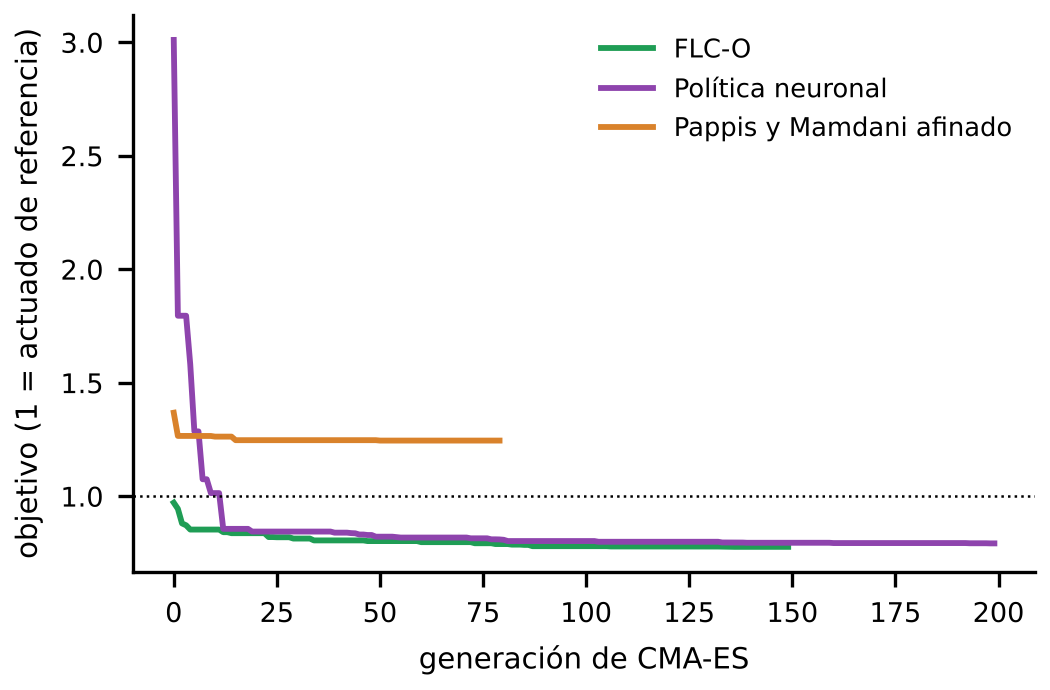
\includegraphics[width=0.9\textwidth]{fig_opt_aprendizaje.png}
\caption{Mejor valor del objetivo $J(\theta)$ por generación para los modelos finales (1: igual al actuado afinado de referencia; menos es mejor).}
\label{fig:aprendizaje}
\end{figure}

\subsection{Tres grupos de escenarios que nunca se mezclan}
\label{sec:datos}
Para que el resultado no sea un ajuste a los datos, cada decisión usa un grupo distinto:

\begin{center}
\small
\begin{tabular}{@{}p{3.3cm}p{5.5cm}p{3.1cm}p{3.2cm}@{}}
\toprule
Grupo & Contenido & Semillas & Para qué se usa \\
\midrule
Entrenamiento & 64 pares de caudales sorteados (cada brazo $\ge180$, suma de 540 a 3300\,veh/h), 3600\,s & 100000 a 100063 & Calcular $J$ y entrenar \\
Validación & 64 pares distintos, 7200\,s & 200000 a 200063 & \textbf{Elegir} entre candidatos, el verde mínimo y la semilla \\
Prueba oficial & Los 16 pares de la Tabla VIII del original $\times$ 20 réplicas, 7200\,s & 0 a 19 & Resultado principal \\
Prueba: no vistos & 64 pares sorteados con otras semillas, 7200\,s & 500000 en adelante & Que no dependa de los 16 pares \\
Prueba: variable & 64 escenarios con demanda que cambia cada 600\,s (factor de 0.4 a 1.6), 7200\,s & -- & Demanda no estacionaria \\
Prueba: saturado & 32 pares con suma de 3000 a 3300\,veh/h, 7200\,s & 400000 en adelante & Cerca de la capacidad \\
\bottomrule
\end{tabular}
\fuente{\texttt{codigo/opt\_entrenar.py} y \texttt{codigo/opt\_evaluar.py}; hiperparámetros en el suplemento del artículo.}
\end{center}
Ningún conjunto de entrenamiento incluye los 16 pares de la Tabla VIII. Las elecciones de diseño (candidato, verde mínimo y semilla) se hicieron con la validación y no con la prueba, y los modelos finales no se reentrenaron a partir de los resultados de prueba. Los conjuntos de prueba se evaluaron con todos los candidatos, no solo con el elegido.

\subsection{Rivales justos}
\label{sec:referencias}
Una mejora solo vale frente a un rival serio. Por eso, además del ciclo fijo de Webster y del actuado de la réplica, se afinaron dos controladores de la literatura con los mismos escenarios de entrenamiento, el mismo rango de verde mínimo (3 a 7\,s) y el mismo verde máximo (hasta 90\,s) que los controladores aprendidos:
\begin{itemize}
\item \textbf{Actuado afinado:} se probaron 45 configuraciones (hueco de 1 a 3\,s, verde mínimo de 3 a 7\,s, máximo de 57, 80 y 90\,s). Resultó hueco de 1\,s, mínimo de 3\,s y máximo de 90\,s, con un $J$ de \JActAfRatio{} respecto del actuado original: ya es un \JActAfMejora\,\% mejor que el original. Es el rival fuerte del artículo.
\item \textbf{Presión máxima} \cite{Varaiya2013}: afinada igual, da \DelayOfMax{}\,s/veh. En este modelo, con dos fases y tiempo perdido, rinde peor que el actuado; se incluye como referencia de la literatura, no como rival fuerte.
\item \textbf{Cota por programación dinámica} \cite{Puterman1994}: la política óptima para caudales \emph{conocidos} y sin ver llegadas futuras. Da \DelayOfMdp{}\,s/veh y se valida contra la simulación de su propia política (diferencia máxima \PdMaxDif\,\%). Sirve como comprobación de coherencia (Sec.~\ref{sec:evidencias}).
\end{itemize}
\textbf{Un error que se detectó y corrigió.} La primera rejilla del actuado exigía un verde mínimo de 5\,s o más, lo que lo debilitaba frente a controladores que podían usar 3\,s y favorecía al propuesto. Se amplió el rango a 3--7\,s y el actuado mejoró un 5\,\% en el conjunto oficial; todas las cifras del artículo usan esta versión justa. Lo mismo se hizo con la presión máxima. Las rejillas anteriores se conservan en \texttt{resultados/opt/actuado\_afinado\_v1.json} y \texttt{resultados/opt/maxpressure\_afinado\_v1.json}.

% =============================================================================
\section{Qué candidatos se probaron}
\label{sec:candidatos}

Se entrenaron, con las mismas condiciones, cinco familias. Cada una responde a una pregunta distinta:

\begin{description}[leftmargin=0pt,labelindent=0pt,itemsep=3pt]
\item[A. Pappis y Mamdani afinado (30 parámetros).] \emph{¿Basta con ajustar el controlador de 1977?} Conserva sus 25 reglas y su estructura y afina el umbral de decisión, una escala y un desplazamiento de las entradas $A$ y $Q$, y un desplazamiento del conjunto de tiempo de cada regla. Con los valores del original reproduce exactamente al controlador replicado. Resultado: \DelayOfPapAf{}\,s/veh (una mejora de \RedPapAf\,\% respecto de Pappis y Mamdani) y, cerca de la saturación, \DelaySaPapAf{}\,s/veh, más del doble que el actuado afinado: con la estructura de 1977 conservada, ajustar ayuda pero no es suficiente.
\item[B. Difuso nuevo de 27 reglas con horizontes fijos (36 parámetros).] \emph{¿Ayuda cambiar la estructura: decidir cada segundo, con menos reglas?} Tres variables (demanda en verde $G$, presión en rojo $R$, verde transcurrido $V$) con tres conjuntos cada una. Resultado: \DelayOfFijos{}\,s/veh; ya supera con holgura a la familia A.
\item[C. Difuso de 81 reglas con el hueco desde la última llegada (93 parámetros).] \emph{¿Más reglas y más información mejoran?} Agrega como cuarta variable el tiempo desde la última llegada al brazo con verde, la señal que usa el actuado. Resultado: \DelayOfReglas{}\,s/veh, sin mejora; la información adicional no aporta y los parámetros se triplican.
\item[D. FLC-O (42 parámetros).] \emph{¿Se puede aprender también cuánto mirar hacia adelante?} Es la familia B con una modificación: las llegadas previstas que alimentan $G$ y $R$ son una combinación lineal, con pesos no negativos \emph{aprendidos}, de las llegadas de los próximos 2, 5 y 10\,s (verde) y 3, 6 y 10\,s (rojo). Resultado: \DelayOfSemCero{}\,s/veh con la misma semilla que B, y \DelayOfFlc{} con la semilla elegida.
\item[E. Política neuronal (121 parámetros).] \emph{¿Cuánto se pierde por exigir reglas legibles?} Una red de una capa oculta con 8 neuronas que recibe 12 características y decide cada segundo. No es un controlador propuesto, sino una referencia de lo que logra un aprendizaje sin estructura con la misma información, también con sus variantes sin vista adelante (causales).
\end{description}

% Generado por gen_justificacion.py (no editar a mano)
\begin{table*}[t]
\centering
\caption{Candidatos entrenados con las mismas condiciones: $J$ de entrenamiento (3600\,s, 64 escenarios) y de validación (7200\,s, 64 escenarios distintos; 1 es igual al actuado afinado, menos es mejor) y retardo medio en los cuatro conjuntos de prueba (s/veh)}
\label{tab:jmodelos}
\footnotesize
\setlength{\tabcolsep}{3.5pt}
\begin{tabular}{@{}p{5.3cm}rcrrrrrr@{}}
\toprule
Candidato & Par. & Vista & $J$ entr. & $J$ val. & Oficial & No vistos & Variable & Saturado \\
\midrule
Actuado afinado (referencia) & 3 & no & -- & 1 & 9.63 & 9.17 & 8.07 & 24.13 \\
Pappis y Mamdani (1977) & 0 & 10 s & -- & -- & 10.95 & 10.40 & 8.65 & 105.87 \\
\midrule
Pappis y Mamdani afinado (25 reglas) & 30 & 10 s & 1.246 & 1.420 & 9.67 & 9.30 & 8.06 & 58.11 \\
\midrule
Difuso 27 reglas, horizontes fijos & 36 & 10 s & 0.826 & 0.837 & 8.44 & 7.88 & 6.56 & 24.80 \\
Difuso 81 reglas con hueco & 93 & 10 s & 0.827 & 0.838 & 8.47 & 7.93 & 6.55 & 25.00 \\
\midrule
FLC-O, $g_{\min}=7$\,s & 42 & 10 s & 0.860 & 0.899 & 8.60 & 8.14 & 6.85 & 25.15 \\
FLC-O, $g_{\min}=5$\,s & 42 & 10 s & 0.815 & 0.834 & 8.21 & 7.75 & 6.41 & 25.16 \\
FLC-O, $g_{\min}=4$\,s & 42 & 10 s & 0.795 & 0.807 & 8.04 & 7.58 & 6.20 & 24.38 \\
FLC-O, $g_{\min}=3$\,s, semilla 0 & 42 & 10 s & 0.794 & 0.805 & 8.00 & 7.51 & 6.21 & 24.79 \\
FLC-O, $g_{\min}=3$\,s, semilla 1 & 42 & 10 s & 0.788 & 0.807 & 8.04 & 7.49 & 6.24 & 24.63 \\
\textbf{FLC-O, $g_{\min}=3$\,s, semilla 2 (elegido)} & 42 & 10 s & 0.777 & 0.800 & 7.91 & 7.40 & 6.07 & 24.29 \\
\midrule
Política neuronal & 121 & 10 s & 0.793 & 0.809 & 8.09 & 7.53 & 6.24 & 25.10 \\
\midrule
Difuso 27 reglas, causal & 36 & no & 0.982 & 1.065 & 9.97 & 9.37 & 8.41 & 25.74 \\
Política lineal causal & 16 & no & 0.949 & 0.992 & 9.53 & 8.97 & 8.10 & 25.11 \\
Política neuronal causal & 121 & no & 0.942 & 0.982 & 9.46 & 8.95 & 8.05 & 24.29 \\
\bottomrule
\end{tabular}
\fuente{\texttt{resultados/opt/evaluacion\_final.json} (prueba), \texttt{codigo/opt\_validar.py} (validación) y campo \texttt{fitness\_train} de cada modelo de \texttt{resultados/opt/} (entrenamiento); tabla generada por \texttt{codigo/gen\_justificacion.py}.}
\end{table*}


% =============================================================================
\section{Por qué se eligió FLC-O}
\label{sec:porque}

\subsection{Los criterios}
Los dos primeros decidieron la elección y se aplicaron con la validación; los otros tres son comprobaciones con los conjuntos de prueba. En orden: (1) mejor $J$ en validación; (2) a igual rendimiento, preferir el modelo con menos parámetros y con reglas que puedan leerse; (3) que la ventaja se mantenga en datos no vistos y con demanda variable; (4) que no se degrade cerca de la saturación; (5) que no dependa de la semilla de entrenamiento.

\subsection{Las razones}
\begin{enumerate}
\item \textbf{Fue el mejor en el grupo reservado para elegir.} En validación, \FLC{} con $g_{\min}=3$\,s y la semilla 2 tiene $J=\JValFlc$, contra \JValMlp{} de la red neuronal, \JValFlcsFijos{} y \JValFlcsGap{} de las otras dos familias difusas y \JValPapAf{} de Pappis y Mamdani afinado (Tabla~\ref{tab:jmodelos}). La elección se hizo con esta columna, no con la de prueba.
\item \textbf{La legibilidad no cuesta rendimiento.} \FLC{} no es peor que una red con 121 parámetros: \DelayOfFlc{} contra \DelayOfMlp{}\,s/veh en el conjunto oficial. Comparados por par de caudales con Wilcoxon pareado y corrección de Holm, \FLC{} es significativamente mejor en \JFlcMlpMejor{} de 16 pares y en ninguno es peor (diferencia media de \JFlcMlpMedia\,\%). El margen es pequeño y hay una asimetría que conviene decir: \FLC{} es la mejor de tres semillas y la red es un solo entrenamiento; con el promedio de las tres semillas (\JSemMedia{}\,s/veh) la ventaja sobre la red sigue, pero baja a \JRedMlpSem\,\%. No se afirma que \FLC{} sea mejor que cualquier red posible (Sec.~\ref{sec:limites}); lo que sí muestra es que exigir 27 reglas legibles no obliga a rendir menos.
\item \textbf{Aprender la vista adelante aporta.} Con horizontes fijos, el mismo difuso de 27 reglas da \DelayOfFijos{}\,s/veh; con los pesos aprendidos, \DelayOfSemCero{} con la misma semilla.
\item \textbf{Más reglas no ayudan.} La variante de 81 reglas da \DelayOfReglas{}\,s/veh. Con 27 reglas, la base se puede leer entera en una tabla (Tabla~\ref{tab:reglasflc}).
\item \textbf{Generaliza.} El retardo de \FLC{} es \JRazOf{} veces el del actuado afinado en el conjunto oficial, \JRazNv{} en los caudales no vistos y \JRazVa{} con demanda variable. La brecha entre $J$ de entrenamiento (\JTrFlc) y de validación (\JValFlc) es de \JBrecha\,\%, pequeña para un modelo de 42 parámetros.
\item \textbf{No se degrada cerca de la saturación.} \DelaySaFlc{}\,s/veh frente a \DelaySaActAf{} del actuado afinado: empate. Pappis y Mamdani da \DelaySaPap{} y su versión afinada \DelaySaPapAf{}.
\item \textbf{No depende de una semilla afortunada.} Se entrenó con tres semillas: en el conjunto oficial dan \JSemCero{} (semilla 0), \JSemUno{} (semilla 1) y \DelayOfFlc{}\,s/veh (semilla 2, la elegida). Si en lugar de la elegida por validación se tomara el promedio de las tres (\JSemMedia{}\,s/veh), la reducción frente a Pappis y Mamdani sería de \JRedSemMedia\,\%, y con la peor, de \JRedSemPeor\,\%; la conclusión no cambia.
\end{enumerate}

\subsection{Cómo se eligió la configuración final}
\begin{itemize}
\item \textbf{Verde mínimo:} se entrenó \FLC{} con 3, 4, 5 y 7\,s y se eligió con la validación: $J=\JValFlcCero$ (3\,s), \JValGCuatro{} (4\,s), \JValGCinco{} (5\,s) y \JValGSiete{} (7\,s). Es el factor que más pesa. Si la norma local exige más de 3\,s, con 5\,s se conserva casi toda la mejora (\DelayOfGCinco{}\,s/veh, \RedPapGCinco\,\% menos que Pappis y Mamdani).
\item \textbf{Semilla:} de las tres semillas con 3\,s ($J=\JValFlcCero$, \JValFlcUno{} y \JValFlc{}) se tomó la de menor $J$ en validación. Esa semilla resultó también la de menor retardo en la prueba, pero la elección no se hizo mirándola.
\item \textbf{Verde máximo de 90\,s:} permite a los controladores aprendidos no depender del tope de 57\,s de 1977, que limita a Pappis y Mamdani cerca de la saturación; el actuado afinado recibió el mismo tope.
\end{itemize}

% =============================================================================
\section{Qué aprendió FLC-O (lectura del modelo)}
\label{sec:lectura}

Las 27 reglas tienen la forma «si $G$ es $\mathcal{G}_i$ y $R$ es $\mathcal{R}_j$ y $V$ es $\mathcal{V}_k$ entonces $c_{ijk}$»; la salida es
\begin{equation}
u=\frac{\sum_{ijk}w_{ijk}\,c_{ijk}}{\sum_{ijk}w_{ijk}},\qquad \text{cambiar de fase}\iff u>0,
\label{eq:salida}
\end{equation}
con $w_{ijk}$ el producto de las tres pertenencias. \emph{Origen:} es el centro de gravedad de consecuentes de un solo punto, un sistema de Mamdani con salidas \emph{singleton} equivalente a uno de Takagi y Sugeno de orden cero \cite{TakagiSugeno1985}. Se eligió esta forma porque da una salida suave, que facilita el trabajo de CMA-ES, y a la vez cada regla dice con un número si conviene cambiar ($c>0$) o seguir ($c<0$).

Las entradas son $G=Q_g+\sum_k\omega_k W_g(l_k)$ y $R=Q_r+\sum_k\rho_k W_r(l'_k)$, con $Q_g$ y $Q_r$ las colas de los brazos en verde y en rojo, $W(l)$ las llegadas previstas en los $l$ segundos siguientes ($l=2,5,10$ en verde y $l'=3,6,10$ en rojo) y $\omega_k,\rho_k\ge0$ pesos que aprende el entrenamiento; $V$ son los segundos de verde transcurridos. Los pesos aprendidos son $\omega=(\JAlfaA,\JAlfaB,\JAlfaC)$ y $\rho=(\JBetaA,\JBetaB,\JBetaC)$. Como cada ventana contiene a la anterior, el peso efectivo de un vehículo según su segundo de llegada es:

\begin{center}
\small
\begin{tabular}{@{}lccc@{}}
\toprule
 & primeros segundos & segundos intermedios & segundos lejanos \\
\midrule
Verde ($G$) & s 1--2: \JWgA{} & s 3--5: \JWgB{} & s 6--10: \JWgC{} \\
Rojo ($R$) & s 1--3: \JWrA{} & s 4--6: \JWrB{} & s 7--10: \JWrC{} \\
\bottomrule
\end{tabular}
\fuente{cálculo sobre los pesos del modelo \texttt{resultados/opt/flcopt\_g3\_s2.json}, hecho por \texttt{codigo/gen\_justificacion.py}.}
\end{center}
\textbf{Interpretación} (una lectura del resultado, no una demostración): para decidir si seguir en verde importan sobre todo los vehículos que llegarán en los próximos 2\,s, que son los que aún aprovecharían el verde; para estimar la presión en rojo importan los que llegarán en los próximos 6\,s, un horizonte parecido a los 5\,s de tiempo perdido de cada cambio de fase. Los conjuntos aprendidos tienen sus nudos en $G=(\JKGA,\JKGB,\JKGC)$, $R=(\JKRA,\JKRB,\JKRC)$ y $V=(\JKVA,\JKVB,\JKVC)$\,s. De los 27 consecuentes, \JNPos{} empujan a cambiar y \JNNeg{} a seguir, con valores de \JCMin{} a \JCMax{}. El patrón es el esperable: se cambia cuando ya queda poca demanda en verde y hay presión en rojo (fila $G$ bajo, $R$ medio: de $+1.45$ a $+2.37$), se sigue cuando la demanda en verde es media o alta (por ejemplo $G$ alto, $R$ medio: de $-3.32$ a $-1.81$), y también cuando ambos brazos están muy cargados, para no malgastar tiempo perdido.

\begin{figure}[t]
\centering
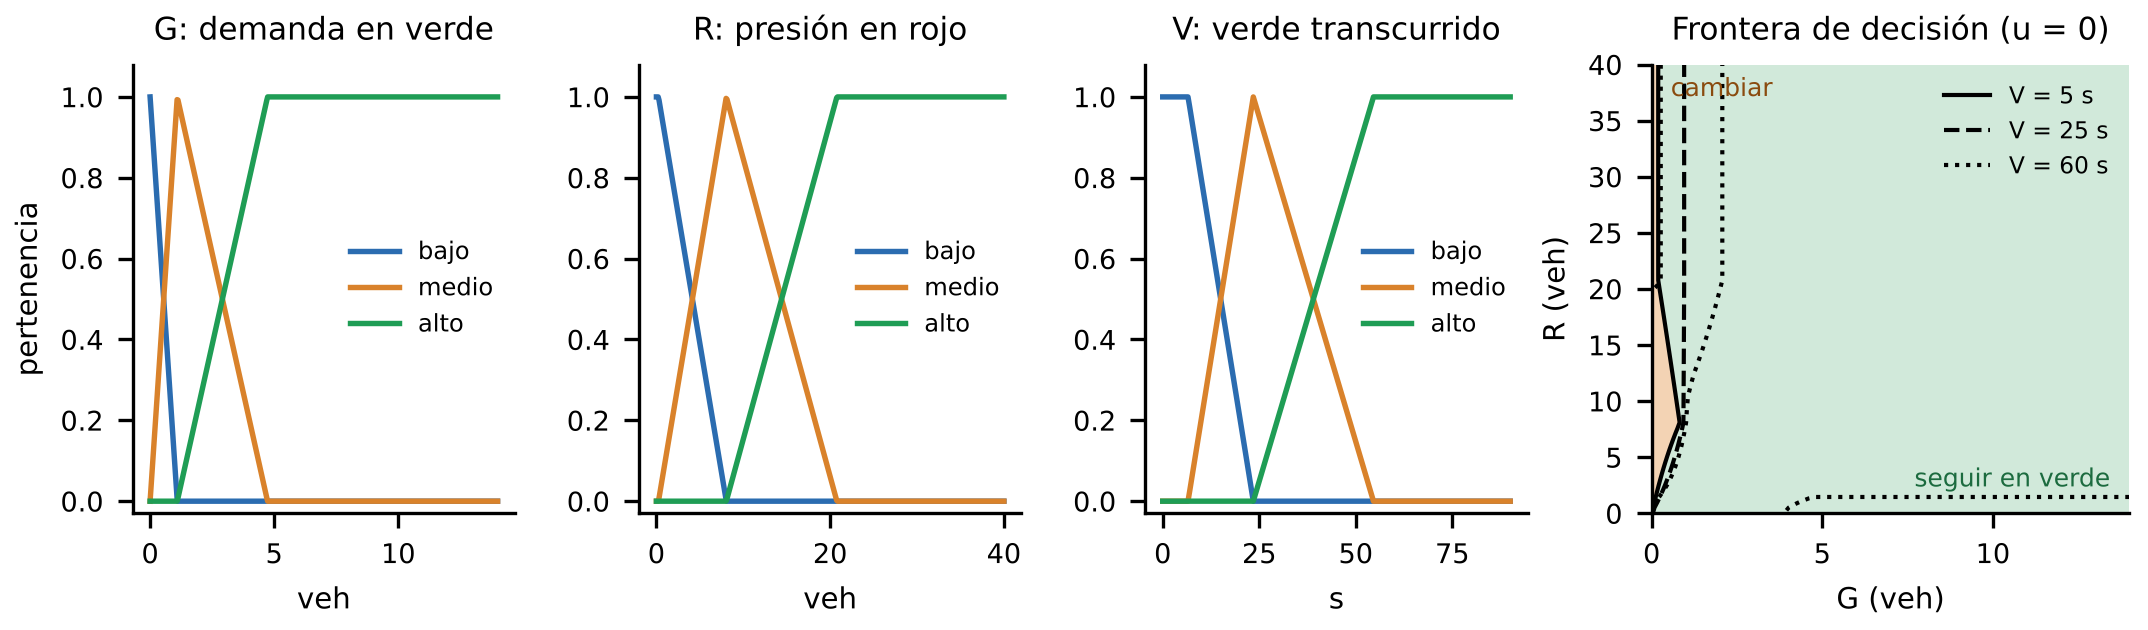
\includegraphics[width=\textwidth]{fig_opt_difuso.png}
\caption{Funciones de pertenencia aprendidas de \FLC{} para $G$, $R$ y $V$ y frontera de decisión $u=0$ en el plano $(G,R)$ para tres valores de $V$.}
\label{fig:difuso}
\end{figure}

\begin{table}[t]
\centering
\caption{Base de reglas de FLC-O: consecuente num\'erico $c_{ijk}$ de cada regla (positivo: cambiar la fase; negativo: seguir en verde) seg\'un la demanda en verde $G$, la presi\'on en rojo $R$ y el verde transcurrido $V$. Nudos $(k_1,k_2,k_3)$: $G$ (0.000, 1.095, 4.731), $R$ (0.239, 8.048, 20.776), $V$ (6.562, 23.457, 54.569). Pesos aprendidos de la vista adelante: verde (0.88, 0.21, 0.03) para 2, 5 y 10 s; rojo (0.22, 0.88, 0.49) para 3, 6 y 10 s.}
\label{tab:reglasflc}
\scriptsize
\begin{tabular}{@{}llrrr@{}}
\toprule
$G$ & $R$ & $V$ bajo & $V$ medio & $V$ alto \\
\midrule
bajo & bajo & +0.06 & +0.04 & $-$0.16 \\
bajo & medio & +1.52 & +1.45 & +2.37 \\
bajo & alto & +0.34 & +2.18 & $-$0.19 \\
medio & bajo & $-$2.75 & $-$1.06 & $-$1.09 \\
medio & medio & $-$0.51 & $-$0.27 & $-$0.20 \\
medio & alto & $-$1.61 & $-$0.36 & +0.60 \\
alto & bajo & $-$0.52 & $-$1.34 & +0.33 \\
alto & medio & $-$3.32 & $-$2.08 & $-$1.81 \\
alto & alto & $-$2.04 & $-$0.03 & $-$1.62 \\
\bottomrule
\end{tabular}
\fuente{modelo entrenado flcopt\_g3\_s2 (resultados/opt/flcopt\_g3\_s2.json).}
\end{table}


% =============================================================================
\section{Evidencias de que la mejora es real}
\label{sec:evidencias}

\begin{enumerate}
\item \textbf{Datos separados.} Entrenar, elegir y probar usan escenarios y semillas distintos (Sec.~\ref{sec:datos}).
\item \textbf{Significancia estadística por par.} En el conjunto oficial, \FLC{} es significativamente mejor que Pappis y Mamdani en \ParMejorPap{} de 16 pares y que el actuado afinado en \ParMejorActAf{}, con corrección de Holm y sin ningún par peor (Wilcoxon pareado sobre 20 réplicas con números aleatorios comunes).
\item \textbf{Datos no vistos y demanda variable.} La reducción se mantiene: \RedPapNv\,\% y \RedActAfNv\,\% con 64 caudales no vistos; \RedPapVa\,\% y \RedActAfVa\,\% con demanda variable.
\item \textbf{Simulador exacto.} El simulador rápido da, escenario por escenario, el mismo retardo que el de referencia, así que ninguna ventaja viene de una simplificación del simulador.
\item \textbf{Comprobación de coherencia con la cota.} La cota por programación dinámica (\DelayOfMdp{}\,s/veh) es el mejor retardo posible para quien conoce los caudales pero no ve el futuro. Todos los controladores \emph{sin} vista adelante quedan por encima: la política neuronal causal da \DelayOfMlpC{}, la lineal causal \DelayOfLinC{}, el actuado afinado \DelayOfActAf{} y el difuso causal \DelayOfFlcC{}. Es coherente con un entrenamiento que no explota atajos del simulador (no lo demuestra, pero un controlador sin vista adelante por debajo de la cota habría sido una señal de alarma). \FLC{} queda por debajo de la cota porque sí ve las llegadas de los próximos segundos, no porque la cota falle.
\item \textbf{Rivales afinados con el mismo presupuesto}, y un error de rejilla que se corrigió en contra del propuesto (Sec.~\ref{sec:referencias}).
\item \textbf{Todo es reproducible} desde el repositorio (Sec.~\ref{sec:repro}).
\end{enumerate}

\begin{figure}[t]
\centering
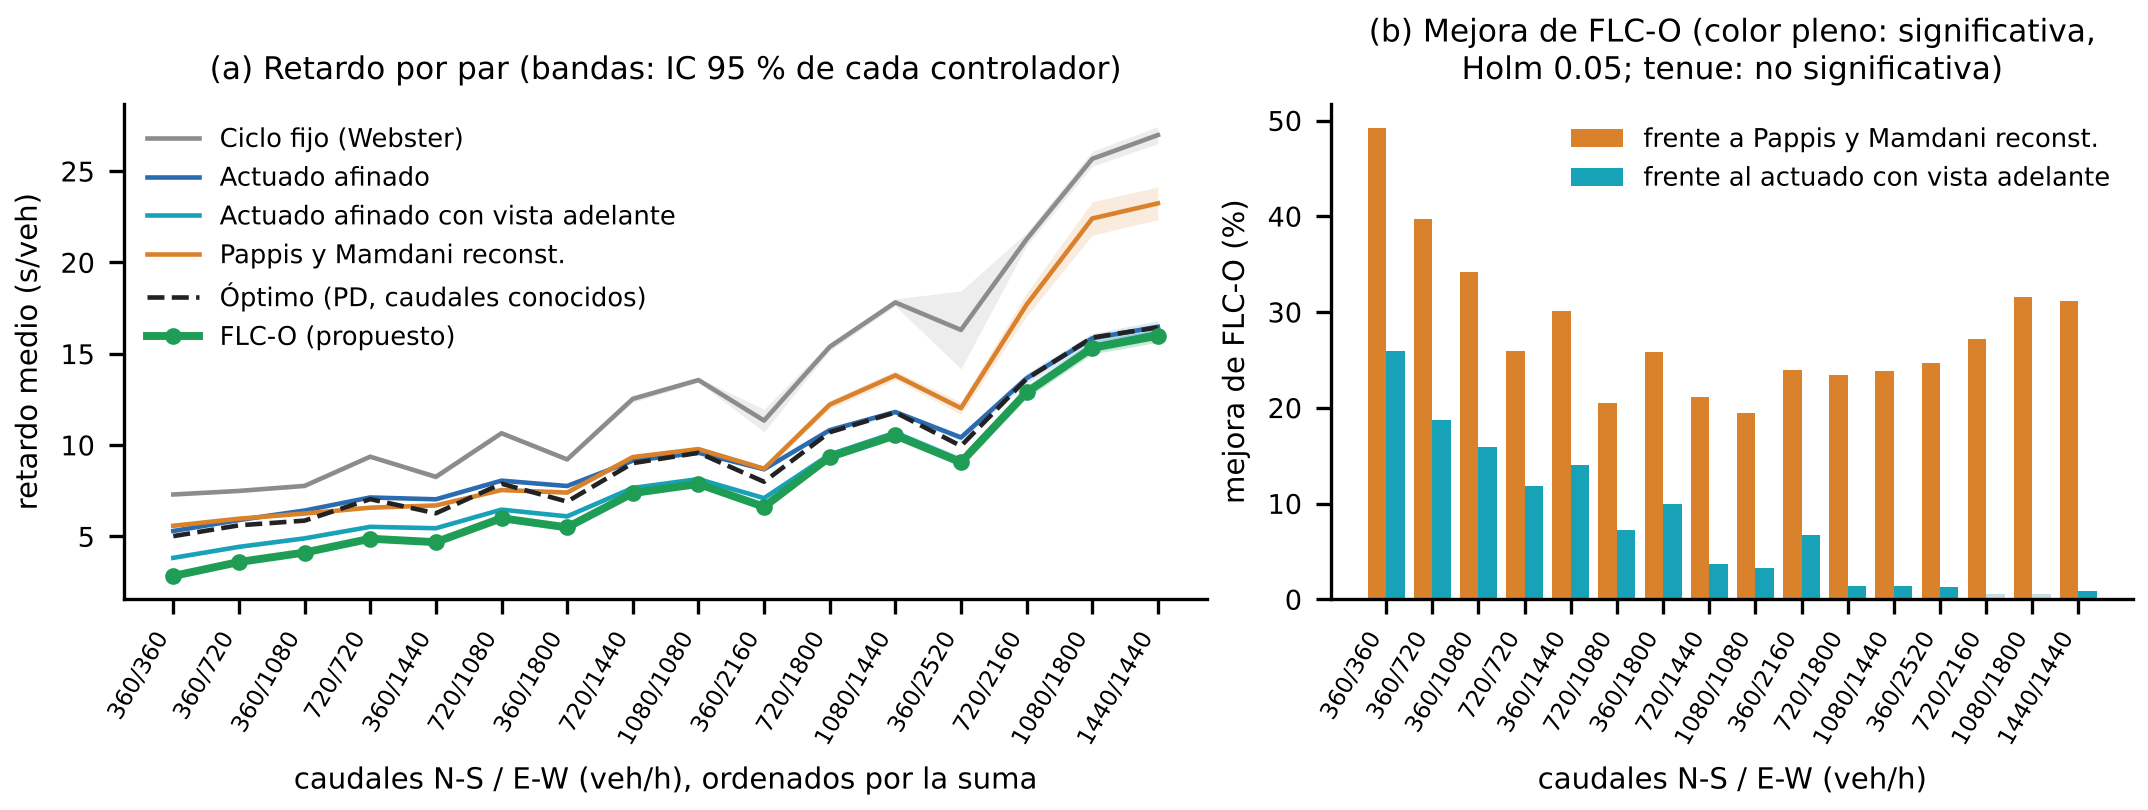
\includegraphics[width=\textwidth]{fig_opt_retardo.png}
\caption{(a) Retardo medio por par de caudales de la Tabla VIII (7200\,s, 20 réplicas); la banda es el intervalo de confianza de 95\,\% de \FLC{}. (b) Mejora de \FLC{} frente a Pappis y Mamdani en cada par; en verde, las significativas con la corrección de Holm.}
\label{fig:retardo}
\end{figure}

% =============================================================================
\section{Qué se corrigió y se descartó en el camino}
\label{sec:camino}

Se deja constancia porque ayuda a juzgar el procedimiento:
\begin{itemize}
\item \textbf{Rejilla del actuado} que favorecía al propuesto: corregida (Sec.~\ref{sec:referencias}).
\item \textbf{La red neuronal ya no se presenta como cota.} Una versión anterior del texto la llamaba «cota»; \FLC{} la iguala o supera, así que solo es una referencia empírica.
\item \textbf{Saturación.} Al principio los controladores entrenados con caudales de hasta 3000\,veh/h se degradaban cerca de la capacidad; entrenar con hasta 3300 lo evitó. El resultado final es empate con el actuado afinado, y así se declara; no se presenta como mejora.
\item \textbf{Verde mínimo de 7\,s.} Los primeros entrenamientos lo usaban y limitaban a los modelos (con 7\,s, \FLC{} da \DelayOfGSiete{}\,s/veh); se estudió el rango de 3 a 7\,s con la validación.
\item \textbf{El hueco desde la última llegada} no ayudó (familia C), pese a ser la señal del actuado.
\item \textbf{Modelos exploratorios} con otras condiciones se conservan en \texttt{resultados/opt/previos/} por transparencia; no se usan en el artículo ni son comparables.
\end{itemize}

% =============================================================================
\section{Limitaciones}
\label{sec:limites}

\begin{enumerate}
\item \textbf{Vista adelante.} \FLC{} usa las llegadas de los próximos 10\,s, un supuesto del original (equivale a detectores aguas arriba sin error). Sin ella, \FLC{} causal da \DelayOfFlcC{}\,s/veh, peor que el actuado afinado (\DelayOfActAf{}); la mejor variante causal, la red neuronal, lo supera solo en \RedActMlpC\,\%. Con vista adelante, \FLC{} tiene un retardo \JGanaVista\,\% menor que el de la mejor variante sin ella (\DelayOfMlpC{}\,s/veh). Es la limitación más importante: en la práctica los detectores tienen error y alcance limitado, y no se midió la robustez ante eso.
\item \textbf{Saturación.} Empate con el actuado afinado, no mejora.
\item \textbf{Verde mínimo de 3\,s.} Puede no ser admisible por seguridad o norma; con 5\,s el resultado es \DelayOfGCinco{}\,s/veh.
\item \textbf{Simulación.} Un cruce aislado, llegadas de Bernoulli, flujo de saturación fijo, sin giros, peatones ni redes. Los parámetros se entrenan y se evalúan en el mismo simulador, aunque con caudales y semillas distintos. No hay datos de campo. Los modelos exploratorios (Sec.~\ref{sec:camino}) guiaron el diseño de las familias de candidatos; por eso las decisiones finales se tomaron con la validación y se reportan todas las variantes, incluidas las peores.
\item \textbf{Alcance de las comparaciones.} El actuado afinado y la presión máxima se afinaron con rejillas finitas; no hay garantía de que sean los mejores de su clase. La red neuronal es de una arquitectura y un entrenamiento; otra podría superarla. No se comparó CMA-ES con otros optimizadores.
\item \textbf{Medida.} El retardo corregido no es el que imprimía el original, así que las cifras no son comparables con las de su Tabla VIII.
\end{enumerate}

% =============================================================================
\section{Preguntas que podrían hacerse}
\label{sec:preguntas}

\begin{description}[leftmargin=0pt,labelindent=0pt,itemsep=4pt]
\item[¿Por qué no usar directamente la red neuronal?] Rinde igual o peor (\DelayOfMlp{} contra \DelayOfFlc{}\,s/veh; \FLC{} es significativamente mejor en \JFlcMlpMejor{} de 16 pares), tiene tres veces más parámetros y no se puede leer ni auditar. Para un semáforo, que alguien pueda revisar por qué cambia de fase es una ventaja práctica.
\item[¿Por qué CMA-ES y no un algoritmo genético u otro?] Porque el objetivo es una simulación sin derivadas y CMA-ES es un método estándar para ese tipo de problema con decenas de parámetros \cite{Hansen2016}. No se comparó con otros; no se afirma que sea el mejor, solo que funciona y converge (Fig.~\ref{fig:aprendizaje}).
\item[¿Cómo sabemos que no hay sobreajuste?] Porque se eligió con la validación y se probó en otros cuatro conjuntos; la brecha entre entrenamiento y validación es de \JBrecha\,\%, y la ventaja se mantiene con caudales no vistos (\JRazNv{} veces el actuado afinado) y con demanda variable (\JRazVa).
\item[¿Por qué el retardo no coincide con la Tabla VIII del original?] Porque se cuenta también la espera de los vehículos que siguen en cola al final. El original no lo hacía. Las cifras de Pappis y Mamdani del artículo salen de la réplica con esta medida, no de la tabla impresa.
\item[¿Por qué el verde mínimo es de 3\,s?] Porque fue el mejor en validación (Sec.~\ref{sec:porque}). Es una elección de simulación; si hace falta más, con 5\,s la mejora frente a Pappis y Mamdani sigue siendo de \RedPapGCinco\,\%.
\item[¿Por qué el controlador ve el futuro?] Porque el modelo original ya lo supone (las llegadas de los próximos 10\,s). Se mantuvo para comparar en las mismas condiciones y se midió cuánto depende de ello, que es mucho.
\item[¿Se puede usar en una intersección real?] No se afirma. Faltan datos de campo, errores de detección y los demás elementos de una intersección real (Sec.~\ref{sec:limites}).
\item[¿Por qué 27 reglas?] Porque con tres conjuntos por variable ($3^3$) la base es la más pequeña que distingue demanda baja, media y alta; con 81 reglas no hubo mejora (familia C).
\end{description}

% =============================================================================
\section{Reproducción y dónde está cada cosa}
\label{sec:repro}

Con Python 3.13 y NumPy 2.5, desde la carpeta del proyecto:
\begin{itemize}
\item \texttt{python codigo/ejecutar\_pruebas.py}: todas las comprobaciones.
\item \texttt{python codigo/opt\_validar.py} seguido de los nombres de los modelos: ordena candidatos con la validación.
\item \texttt{python codigo/opt\_evaluacion\_final.py}: los cuatro conjuntos de prueba y la estadística.
\item \texttt{python codigo/gen\_tablas\_opt.py} y \texttt{python codigo/gen\_justificacion.py}: las cifras y tablas del artículo y de este documento.
\end{itemize}

\begin{center}
\small
\begin{tabular}{@{}R{5.2cm}R{10.2cm}@{}}
\toprule
Qué & Dónde \\
\midrule
Simulador vectorizado y su prueba de equivalencia & \texttt{codigo/sim\_batch.py}, \texttt{codigo/test\_sim\_batch.py} \\
Controladores (Pappis y Mamdani afinado, difusos, política neuronal, referencias) & \texttt{codigo/opt\_controladores.py}, \texttt{opt\_flc.py}, \texttt{opt\_flc2.py}, \texttt{opt\_politicas.py} \\
Optimizador CMA-ES & \texttt{codigo/opt\_es.py} \\
Cota por programación dinámica & \texttt{codigo/opt\_mdp.py}, \texttt{resultados/opt/mdp\_oficial.json} \\
Entrenamiento y escenarios & \texttt{codigo/opt\_entrenar.py}, \texttt{opt\_entrenar\_modelo.py} \\
Modelos entrenados y el elegido & \texttt{resultados/opt/flcopt\_g3\_s2.json} (el elegido) y \texttt{resultados/opt/modelos\_finales.json} \\
Evaluación final y estadística & \texttt{codigo/opt\_evaluacion\_final.py}, \texttt{resultados/opt/evaluacion\_final.json} \\
Rivales afinados & \texttt{resultados/opt/actuado\_afinado.json} y \texttt{resultados/opt/maxpressure\_afinado.json} \\
Simulador interactivo con calle y autos & \texttt{codigo/simulador\_gui.py}, \texttt{codigo/web\_sim.py} \\
Artículo, suplemento y este documento & \texttt{articulo/main.tex}, \texttt{suplemento.tex}, \texttt{justificacion.tex} \\
\bottomrule
\end{tabular}
\fuente{repositorio del proyecto, rama \texttt{main}.}
\end{center}

\bibliographystyle{IEEEtran}
\bibliography{referencias}

\end{document}
